\section{}

\textbf{Tiempo de lectura:} \{s07-reading-time\}

Dado que el sistema operativo y los procesos de usuarios comparten los
recursos del sistema informático, necesitamos estar seguros de que un
error en un programa solo afecte al proceso que lo ejecuta ---por
ejemplo, que un proceso no puede modificar la memoria de otro proceso o
la del núcleo del sistema---. Por eso es necesario establecer mecanismos
de protección frente a los errores en los programas que se ejecutan en
el sistema.

\section{Software controlado mediante
interrupciones}\label{_software_controlado_mediante_interrupciones}

Antes de entender cómo funcionan estos mecanismos de protección debemos
entender que los sistemas operativos modernos pertenecen a un tipo de
software que se dice que está controlado mediante interrupciones.

Los sucesos que requieren la atención del sistema casi siempre se
indican mediante una interrupción:

\begin{itemize}
\item
  Cuando un proceso comete un error ---como una división por cero o un
  acceso a memoria no válido--- lo que se genera es una excepción en la
  CPU. Esta excepción despierta al sistema operativo para que haga lo
  que sea más conveniente.
\item
  Cuando un proceso necesita un servicio lo que hace es lanzar una
  llamada al sistema, que no es más que ejecutar una instrucción que
  lanza una excepción en la CPU. Esta excepción despierta al sistema
  operativo para que atienda la petición.
\item
  Cuando los dispositivos de E/S requieren la atención del sistema
  operativo ---por ejemplo, porque se ha completado una transferencia de
  datos--- se genera una interrupción en la CPU, que despierta al
  sistema operativo.
\end{itemize}

Esto funciona así porque el sistema operativo configura la CPU durante
el arranque para que si ocurre cualquier interrupción o excepción la
ejecución, salte a rutinas en el código del núcleo, con el objeto de
darles el tratamiento adecuado.

Si ningún proceso realiza una acción ilegal o pide un servicio, ni
ningún dispositivo de E/S pide la atención del sistema, el sistema
operativo permanece inactivo esperando a que algo ocurra.

Teniendo todo esto en cuenta podremos entender mejor cómo funciona el
modo dual.

\section{Operación en modo dual}\label{_operaciuxf3n_en_modo_dual}

Para proteger el sistema de programas con errores es necesario poder
distinguir entre la ejecución del código del sistema operativo y del
código de los programas de usuario, de tal forma que el código de los
programas de usuario esté más limitado en lo que puede hacer que el del
sistema operativo.

El método que utilizan la mayor parte de los sistemas operativos
consiste en utilizar algún tipo de soporte en la CPU que permita
diferenciar entre varios modos de ejecución y restringir la utilización
de las instrucciones peligrosas ---llamadas \textbf{instrucciones
privilegiadas}{}--- para que solo puedan ser utilizadas en el modo en el
que se ejecuta el código del sistema operativo.

\subsection{Modos de operación}\label{_modos_de_operaciuxf3n}

Así que como mínimo son necesarios dos modos de operación diferentes:

\begin{itemize}
\item
  En el \textbf{modo usuario}{}, en el que se ejecuta el código de los
  procesos de los usuarios. Si se hace un intento de ejecutar una
  instrucción privilegiada en este modo, el hardware la trata como
  ilegal y genera una excepción que es interceptada por el sistema
  operativo, en lugar de ejecutar la instrucción.
\item
  En el \textbf{modo privilegiado}{} ---también denominado \textbf{modo
  supervisor}{}, \textbf{modo del sistema}{} o \textbf{modo kernel}{}---
  se ejecuta el código de las tareas del sistema operativo. La CPU es la
  encargada de garantizar que las instrucciones privilegiadas solo
  pueden ser ejecutadas en este modo.
\end{itemize}

El modo actual de operación puede venir indicado por un \textbf{bit de
modo}{} en alguno de los registros de configuración de la CPU, de tal
forma que, si por ejemplo, el bit está a 0, la CPU considera que el
código en ejecución opera en modo privilegiado, mientras que si el bit
está a 1, el código en ejecución opera en modo usuario.

Comúnmente en el grupo de las \textbf{instrucciones privilegiadas} se
suelen incluir:

\begin{itemize}
\item
  La instrucción para conmutar al modo usuario desde el modo
  privilegiado.
\item
  Las instrucciones para acceder a dispositivos de E/S.
\item
  Las instrucciones necesarias para la gestión de las interrupciones.
  Por ejemplo, para desactivarlas ---evitando que se lancen---
  activarlas y configurarlas.
\end{itemize}

Aunque para operar en modo dual solo se necesita que la CPU admita los
dos modos descritos, existen procesadores que soportan más, con la idea
de tener mayor control sobre el nivel de privilegio en el que se ejecuta
cada componente del sistema.

Es el caso de la arquitectura Intel x86, que soporta 4 modos de
operación\hyperref[Wikipedia-Anillo]{???}. El modo 0 es para el software
más confiable y el que necesita más privilegios, que generalmente es el
núcleo. Mientras que el modo 3 se utiliza para el software menos
confiable y que necesita más supervisión, que normalmente son los
procesos de usuario.

La idea detrás de tener los modos 1 y 2 es usarlos para controladores de
dispositivo o procesos que dan servicio al resto del sistema. Así estos
componentes pueden tener mayores privilegios que los procesos de usuario
---por ejemplo, los controladores de dispositivo necesitan acceso
directo al hardware--- pero al mismo tiempo serían supervisados y no
podrían afectar al núcleo, que se ejecuta en el modo 0.

Sin embargo, los sistemas operativos con mayor cuota de mercado
---incluyendo Microsoft Windows, macOS, Linux y Android--- solo utilizan
los modos 0 y 3. Los motivos son que los desarrolladores de sistemas no
encuentran realmente ninguna ventaja en utilizar más modos y que
complica portar el sistema operativo a procesadores donde solo se
soporten dos.

En procesadores x86 recientes, que vienen con instrucciones específicas
para facilitar la ejecución de máquinas virtuales, se ha incorporado un
modo -1, para que el núcleo del sistema operativo virtualizado se
ejecute en el modo 0 mientras es supervisado desde el modo -1 por el
núcleo del sistema operativo anfitrión.

En los procesadores x86 es importante no confundir los \textbf{modos
real}{} y \textbf{protegido}{} con el modo dual y los niveles de
privilegio de los que estamos hablando.

Por compatibilidad hacia atrás, los procesadores x86 se inician en modo
real, donde se comportan como una CPU \{intel8086\}. En este modo, por
ejemplo, solo tienen acceso al primer mega de memoria RAM ---ya que los
procesadores \{intel8086\} solo tenían 20 bits para direcciones de
memoria---.

Cuando un sistema operativo moderno arranca, lo primero que hace es
iniciar el modo protegido, en el que se activan todas las
características de la CPU. Entre otras, el direccionamiento de 32 o 64
bits ---según el procesador que sea--- y la posibilidad de usar los 4
niveles de privilegio, de los que hemos hablado, para que el núcleo
pueda supervisar al resto de componentes.

\subsection{Ejecución de
instrucciones}\label{_ejecuciuxf3n_de_instrucciones}

A continuación podemos ver el ciclo de vida de la ejecución de
instrucciones en un sistema con modo dual de operación:

\begin{enumerate}
\def\labelenumi{\arabic{enumi}.}
\item
  Inicialmente, al arrancar el ordenador, la CPU se inicia en el modo
  privilegiado ---es decir, en nuestro ejemplo, con el bit de modo a
  0---. En este modo se carga el núcleo del sistema operativo e inicia
  su ejecución.
\item
  El núcleo del sistema operativo debe cambiar al modo usuario
  ---poniendo el bit de modo a 1--- antes de ceder la CPU a un proceso
  de usuario. Esto ocurre cuando es necesario que un proceso de usuario
  continúe o inicie su ejecución (véase el
  \hyperref[_el_asignador]{???}). Así se asegura que el código de los
  procesos de usuario siempre se ejecuten en modo usuario, con menos
  privilegios.
\item
  La CPU conmuta a modo privilegiado cuando ocurre una interrupción o
  una excepción ---poniendo el bit de modo a 0--- antes de comenzar el
  código del sistema operativo que se encargará de tratarlas.
\end{enumerate}

Esto último es muy importante. Como ya hemos comentado, los sistemas
operativos están controlados mediante interrupciones. Al activarse el
modo privilegiado cada vez que ocurre una interrupción, podemos estar
seguros de que las tareas del sistema operativo se ejecutarán siempre en
modo privilegiado.

Cuando se dispone de la protección del modo dual, el hardware se encarga
de detectar los errores de ejecución y de notificarlo al sistema
operativo mediante excepciones, siendo responsabilidad de este último
realizar un tratamiento adecuado de los mismos. Por lo general, si un
programa falla de alguna forma ---como por ejemplo, intentando utilizar
una instrucción ilegal o de acceder a una zona de memoria inválida--- el
sistema operativo lo hace terminar.

\section{Protección de la memoria}\label{_protecciuxf3n_de_la_memoria}

La memoria principal debe acomodar tanto el sistema operativo como a los
diferentes procesos de los usuarios. Por eso la memoria normalmente se
divide en dos partes o espacios:

\begin{enumerate}
\def\labelenumi{\arabic{enumi}.}
\item
  La primera parte es el \textbf{espacio del núcleo}{}. Sirve para
  albergar el núcleo del sistema operativo.

  El sistema operativo puede estar localizado tanto en la parte baja
  como en la parte alta de la memoria. El factor determinante es la
  dirección de memoria a la que salta la CPU cuando ocurre una
  interrupción o la dirección del vector de interrupciones ---que es una
  tabla en la memoria donde se definen las direcciones a las que saltará
  la CPU en caso de que ocurra una interrupción o una excepción--- según
  esté definido en la arquitectura correspondiente.

  En los procesadores de la familia x86, el vector de interrupciones
  reside en la dirección 0x00000000 y ocupa 0x400 bytes, por lo que,
  normalmente, el sistema operativo se aloja en la parte baja de la
  memoria. Sin embargo, en los procesadores MIPS las interrupciones se
  manejan saltando a la dirección 0x80000180, que está en la mitad del
  espacio de direcciones, en procesadores de 32 bits. Por tanto, lo más
  probable es que se aloje el sistema operativo por encima de la
  dirección 0x80000000.
\item
  La segunda parte es el \textbf{espacio de usuario}{} y alberga los
  procesos de usuario.
\end{enumerate}

Sin embargo, en los sistemas operativos modernos, los procesos no tienen
acceso libre a toda memoria física, con el objeto de proteger a los
procesos en ejecución y al sistema operativo de posibles errores en
cualquiera de ellos:

\begin{itemize}
\item
  El sistema operativo proporciona a cada proceso una «vista» privada de
  la memoria RAM; de tal forma que el \textbf{espacio de usuario} que ve
  cada proceso es similar al que vería cada uno de ellos si se estuviera
  ejecutando en solitario (véase la
  \hyperref[fig-protecciuxf3n-memoria]{Mapeo de la memoria física en el
  espacio de direcciones virtual de un proceso.}).
\item
  A esa «vista» que tiene cada proceso de la memoria es a lo que se
  denomina \textbf{espacio de direcciones virtual}{} del proceso. Está
  formada por el conjunto de todas las direcciones que puede generar la
  CPU para un proceso dado. Por ejemplo, en una CPU de 32 bits el
  espacio de direcciones virtual tiene 4 GiB, desde la dirección
  0x00000000 a 0xFFFFFFFF.
\item
  En los accesos a la memoria principal durante la ejecución del
  proceso, estas \textbf{direcciones virtuales}{} son convertidas por la
  CPU en direcciones físicas, antes de ser enviadas a la memoria
  principal. Por tanto las \textbf{direcciones físicas}{} son las
  direcciones reales que ve la memoria. Mientras que el \textbf{espacio
  de direcciones físico}{} es el conjunto de direcciones físicas que
  corresponden a todas las direcciones virtuales de un espacio de
  direcciones virtual dado.
\end{itemize}

\begin{figure}
\centering
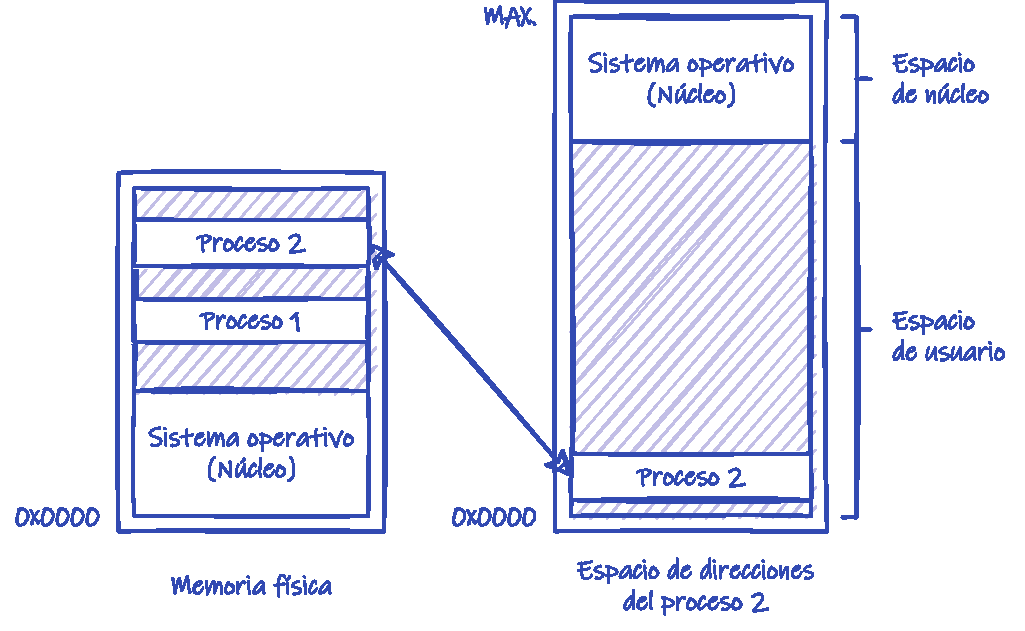
\includegraphics[width=0.8\textwidth]{media/C07_modo_dual/protección_memoria.pdf}
\caption{Mapeo de la memoria física en el espacio de direcciones virtual
de un proceso.}\label{fig-protecciuxf3n-memoria}
\end{figure}

La conversión de una dirección virtual en una física, la realiza en
tiempo de ejecución un componente de la CPU denominado MMU
(\emph{Memory-Management Unit}).

Las ventajas de usar esta técnica, desde el punto de vista de la
protección de la memoria son:

\begin{itemize}
\item
  Permite el aislamiento de los procesos, creando para cada uno la
  ilusión de que toda la memoria es para él y evitando que un proceso
  pueda acceder a la memoria de otros procesos.
\item
  Permite marcar modos de acceso autorizados en las diferentes regiones
  de la memoria ---como por ejemplo lectura, escritura y ejecución---
  evitando que el código ejecutado en modo usuario tenga acceso a zonas
  a las que no debería tenerlo. El acceso a la memoria en un modo no
  autorizado se considera una instrucción privilegiada, por lo que ese
  tipo de acceso desde el modo usuario siempre genera una excepción. Por
  ejemplo, si se intenta ejecutar instrucciones en una zona de memoria
  no marcada con el permiso de ejecución.
\end{itemize}

\section{El temporizador}\label{_el_temporizador}

El \textbf{{}temporizador} se configura por el sistema operativo durante
el arranque del sistema para interrumpir a la CPU a intervalos
regulares. Así, cuando el temporizador interrumpe, el control se
transfiere automáticamente al núcleo del sistema. Entonces este puede:

\begin{itemize}
\item
  Conceder más tiempo al proceso en ejecución.
\item
  Detenerlo y darle más tiempo de CPU en el futuro
\item
  Tratar la interrupción como un error y terminar el programa.
\end{itemize}

El temporizador se utiliza para asegurar que ningún proceso acapara la
CPU indefinidamente. Por ejemplo, un programa mal desarrollado que entra
en un bucle infinito, del que no sale jamás.

Obviamente, las instrucciones que pueden modificar el contenido del
temporizador son instrucciones privilegiadas.

\section{Máquinas virtuales}\label{_muxe1quinas_virtuales}

{} Utilizando las técnicas comentadas anteriormente, el sistema
operativo crea a los procesos la ilusión de que se ejecutan en su propio
procesador y memoria principal, aunque realmente los estén compartiendo
con otros procesos. Obviamente, los procesos saben que hay un sistema
operativo que los supervisa, porque no pueden acceder directamente al
hardware, sino que deben solicitar los distintos recursos a través de
las llamadas al sistema.

Sin embargo, en algunos casos puede interesar que los procesos accedan a
los recursos a través de una interfaz de hardware virtual. Por ejemplo,
que un proceso, en lugar de hacer llamadas al sistema para pedir al
sistema operativo que lea cierto bloque de datos del disco duro, pueda
ejecutar directamente las instrucciones de E/S necesarias para pedir a
la controladora de disco que lea el bloque que le interesa y lo deposite
en la memoria, como si no estuviera siendo supervisado por el sistema
operativo.

Obviamente, no se trata de que el proceso tengo acceso a la controladora
real, sino que en el sistema hay un componente de software que ejecuta
una simulación de algún modelo de controladora de disco al que llegan
las peticiones del proceso. Como las instrucciones de E/S necesarias
para acceder al hardware son instrucciones privilegiadas, el sistema
operativo las intercepta ---gracias al apoyo del modo dual--- pero no
interpreta la situación como debida a un programa defectuoso, sino que
traslada la operación solicitada a los componentes de hardware virtual,
para luego continuar la ejecución del proceso en la siguiente
instrucción. El resultado es que el proceso tiene la ilusión de que se
ejecuta solo en una máquina vacía, con cierto hardware al que puede
acceder directamente, aunque este hardware realmente está siendo
simulado.

Los componentes de hardware virtual simulan el comportamiento de modelos
concretos de dispositivos hardware reales, implementando la
funcionalidad del hardware simulado con ayuda de otros componentes del
sistema operativo. Por ejemplo, una tarjeta de sonido virtualizada, en
última instancia usará los servicios del sistema operativo para
reproducir o grabar sonido usando el dispositivo real, mientras que el
controlador de disco virtualizado probablemente simulará las operaciones
de lectura y escritura trasladándolas a un archivo del sistema de
archivos real que hará de imagen del disco duro virtual.

Estos procesos que no se solicitan servicios al sistema operativo
mediante llamadas al sistema, si no haciendo uso de una interfaz de
hardware virtual, es lo que se conoce como máquinas virtuales. El
software de gestión de las máquinas virtuales es el responsable de
implementar los componentes de hardware virtual y de recibir del sistema
operativo los intentos de ejecutar instrucciones privilegiadas por parte
del código que se ejecuta dentro de las máquinas virtuales. Por tanto,
la operación en modo dual y las técnicas comentadas anteriormente en
este tema son fundamentales para implementar el soporte de máquinas
virtuales en los sistemas operativos modernos.

Una interfaz de hardware virtual es, por lo general, menos eficiente que
una basada en llamadas al sistema. A fin de cuentas, necesita que se
simule el hardware virtual mediante software, para luego traducir las
peticiones realizadas mediante esa interfaz en peticiones al sistema
operativo del sistema anfitrión. Una solución frecuente a este
inconveniente es la \textbf{paravirtualización}.

Por lo general, en la máquina virtual se ejecuta un sistema operativo,
que debe tener controladores de dispositivos para gestionar el acceso al
hardware virtual de la máquina. Es decir, los procesos que se ejecutan
en la máquina virtual solicitan servicios al sistema mediante llamadas
al sistema. El sistema operativo atiende esas peticiones usando los
recursos del hardware virtual, a los que accede mediante los
controladores de dispositivo correspondientes.

La \textbf{{}paravirtualización} consiste en instalar en el sistema
operativo de las máquinas virtuales controladores de dispositivo
desarrollados bajo la premisa de que se van a usar en una máquina
virtual. La particularidad es que estos controladores saben usar una
interfaz que provee el software de gestión de máquinas virtuales
---mediante un mecanismo similar a las llamadas al sistema--- para
trasladar las peticiones que llegan del sistema operativo en la máquina
virtual directamente al sistema operativo anfitrión, sin necesidad de
utilizar el hardware simulado.

\section{Arranque del sistema}\label{_arranque_del_sistema}

Desde el momento en que el ordenador se pone en marcha hasta que el
sistema operativo inicia su ejecución se realizan una serie de
operaciones. Estos son los pasos más comunes en el arranque de un
sistema:

\begin{enumerate}
\def\labelenumi{\arabic{enumi}.}
\item
  Llega a la CPU una señal de RESET motivada por el encendido del
  sistema o por un reinicio.
\item
  La CPU inicializa el contador de programa a una dirección predefinida
  de la memoria. En esa dirección está el \emph{bootstrap} inicial.
\end{enumerate}

El \emph{{}bootstrap} es el programa que se encarga en primera instancia
del arranque. Debe estar almacenado en una memoria no volátil ---ROM o
Flash--- porque la RAM está en un estado indeterminado en el momento del
arranque.

En los PC el \emph{bootstrap} forma parte del \emph{{}firmware} ---sea
BIOS o UEFI--- de las placas madres.

El término \emph{firmware} viene de que por sus características se sitúa
en algún lugar entre el hardware y el software. Concretamente es un
componente de software instalado en un dispositivo hardware para
encargarse de su control a bajo nivel.

\subsection{Tareas del bootstrap}\label{_tareas_del_bootstrap}

El \emph{bootstrap} debe realizar diversas tareas:

\begin{enumerate}
\def\labelenumi{\arabic{enumi}.}
\item
  \textbf{Diagnóstico de la máquina} ---o \emph{Power-on Self-Test}
  (POST)---. El \emph{bootstrap} se detiene en este punto si el sistema
  no supera el diagnóstico.
\item
  \textbf{Inicializar el sistema}. Por ejemplo, configurar los registros
  de la CPU, inicializar los dispositivos y contenido de la memoria,
  etc.
\item
  \textbf{Iniciar el sistema operativo}.
\end{enumerate}

Al iniciar el sistema operativo hay que considerar que puede estar en
diferentes ubicaciones según el tipo de dispositivo:

\begin{itemize}
\item
  En \textbf{consolas de videojuegos, móviles y otros dispositivos
  empotrados} se almacena el sistema operativo en alguna forma de
  memoria de solo lectura ---ROM o Flash---. Como la ejecución en esas
  memorias es más lenta que en la RAM, muchas veces el \emph{bootstrap}
  suele copiar el sistema a la RAM durante el arranque, antes de
  iniciarlo.
\item
  En \textbf{sistemas operativos de gran tamaño} ---incluidos los de
  propósito general--- el sistema se almacena en disco.
\end{itemize}

En los sistemas más antiguos, el \emph{bootstrap} lee de una posición
fija del disco ---generalmente el bloque 0--- el gestor de arranque, lo
copia en la memoria y lo ejecuta. Esto es lo que ocurre en los PC más
antiguos que utilizan BIOS y particiones MBR.

También se llama {}MBR a ese bloque 0 del disco donde está el gestor de
arranque. De hecho MBR son las siglas de \emph{Master Boot Record} o
\href{https://es.wikipedia.org/wiki/Registro_de_arranque_principal}{registro
de arranque principal}.

Aunque en ocasiones el código de ese bloque inicial de arranque sabe
cargar e iniciar el sistema operativo completo, es común que solo sepa
donde está el resto del gestor de arranque en el disco, para cargarlo y
ejecutarlo. No debemos olvidar que el código cargado por el
\emph{bootstrap} debe caber en un solo bloque del disco, que
generalmente tiene solo 512 bytes.

En los PC más modernos que utilizan UEFI y particiones GPT, la UEFI
tiene la capacidad de leer el sistema de archivo en las particiones para
buscar directamente los archivos del gestor de arranque completo. Una
vez el \emph{bootstrap} los encuentra, los carga y ejecuta.

En ambos casos, el gestor de arranque completo es el programa que sabe
cómo iniciar el sistema operativo así que: explora el sistema de
archivos en busca del núcleo del sistema, lo carga e inicia su
ejecución.

A partir de este punto, cada sistema operativo prosigue de forma
diferente. A modo de ejemplo, veremos como prosigue el arranque en
sistemas UNIX en modo texto.

\subsection{Arranque de sistemas UNIX}\label{_arranque_de_sistemas_unix}

Al iniciarse el núcleo del sistema, este realiza una serie de tareas:

\begin{enumerate}
\def\labelenumi{\arabic{enumi}.}
\item
  Configura el sistema para crear un entorno adecuado para la ejecución
  de los procesos: configuración de interrupciones, configuración de los
  modos de ejecución ---privilegiado y usuario--- y de la gestión de la
  memoria; inicialización de dispositivos y controladores; montaje del
  sistema de archivos raíz; creación del proceso inactivo ---que se
  ejecutará cuando no haya nada que hacer--- etc.
\item
  Crea el proceso \textbf{{}init} ---que por ser el primero tiene PID
  1--- a partir de la carga del programa \texttt{init} almacenado en el
  sistema de archivos raíz. En los sistemas GNU/Linux actuales el
  proceso \textbf{init} más común es \{cmd\_systemd\}.
\item
  El planificador de la CPU toma el control de la gestión de la CPU y el
  núcleo se queda dormido. Puesto que la función del planificador es
  asignar procesos a la CPU y solo hay uno, el proceso \textbf{init},
  este es escogido y comienza su ejecución.
\item
  El proceso \textbf{init} lanza los \emph{scripts} encargados de
  configurar los servicios ---también llamados demonios--- del sistema.
  Por ejemplo, para el registro de eventos del sistema, gestión de
  dispositivos, particiones, impresoras, entre otros.
\end{enumerate}

El proceso \textbf{init} también configura el entorno de usuario.
Configura las terminales del sistema, inicia un proceso \textbf{login}
conectado a cada una y se duerme a la espera. Estos procesos
\textbf{login} son monitorizados por \textbf{init} para reiniciarlos en
caso de que mueran.

Aunque, por lo general, un sistema de escritorio tiene una única pareja
de teclado y monitor y, por lo tanto, una única terminal real; el
sistema suele estar configurado para crear varios terminales virtuales
entre los que el usuario puede conmutar usando las combinaciones de
teclas adecuadas.

Los procesos \textbf{login} se encargan de autenticar a los usuarios y
de iniciar y configurar su sesión:

\begin{enumerate}
\def\labelenumi{\arabic{enumi}.}
\item
  Muestran una pantalla de inicio de sesión donde se solicita el nombre
  del usuario y su contraseña.
\item
  Autentican al usuario comprobando las credenciales proporcionadas por
  el mismo.
\item
  Si la autenticación es positiva, el proceso \textbf{login} cambia su
  identidad actual ---generalmente de \emph{root} o administrador del
  sistema--- por la del usuario autenticado, configura la sesión y
  sustituye su programa actual por el del intérprete de comandos que
  tiene configurado ese usuario (véase el
  \hyperref[sect-procesos-posix-api]{???}).
\end{enumerate}

El intérprete de comandos completa la configuración del entorno
basándose en sus archivos de configuración, muestra el
\href{https://es.wikipedia.org/wiki/Prompt}{prompt} y queda a la espera
del primer comando del usuario.
